\documentclass{article}
\usepackage{amsmath}
\usepackage[top=2cm, left=2cm, right=1cm, bottom=2cm]{geometry}
\usepackage{fancyhdr}
\usepackage{graphicx}
\usepackage{longtable}

\usepackage{amsmath,amssymb}
\usepackage{iftex}
\ifPDFTeX
  \usepackage[T1]{fontenc}
  \usepackage[utf8]{inputenc}
  \usepackage{textcomp} % provide euro and other symbols
\else % if luatex or xetex
  \usepackage{unicode-math} % this also loads fontspec
  \defaultfontfeatures{Scale=MatchLowercase}
  \defaultfontfeatures[\rmfamily]{Ligatures=TeX,Scale=1}
\fi
\usepackage{lmodern}
\ifPDFTeX\else
  % xetex/luatex font selection
\fi
% Use upquote if available, for straight quotes in verbatim environments
\IfFileExists{upquote.sty}{\usepackage{upquote}}{}
\IfFileExists{microtype.sty}{% use microtype if available
  \usepackage[]{microtype}
  \UseMicrotypeSet[protrusion]{basicmath} % disable protrusion for tt fonts
}{}
\makeatletter
\@ifundefined{KOMAClassName}{% if non-KOMA class
  \IfFileExists{parskip.sty}{%
    \usepackage{parskip}
  }{% else
    \setlength{\parindent}{0pt}
    \setlength{\parskip}{6pt plus 2pt minus 1pt}}
}{% if KOMA class
  \KOMAoptions{parskip=half}}
\makeatother
\usepackage{xcolor}
\usepackage{longtable,booktabs,array}
\usepackage{calc} % for calculating minipage widths
% Correct order of tables after \paragraph or \subparagraph
\usepackage{etoolbox}
\makeatletter
\patchcmd\longtable{\par}{\if@noskipsec\mbox{}\fi\par}{}{}
\makeatother
% Allow footnotes in longtable head/foot
\IfFileExists{footnotehyper.sty}{\usepackage{footnotehyper}}{\usepackage{footnote}}
\makesavenoteenv{longtable}
\usepackage{graphicx}
\makeatletter
\def\maxwidth{\ifdim\Gin@nat@width>\linewidth\linewidth\else\Gin@nat@width\fi}
\def\maxheight{\ifdim\Gin@nat@height>\textheight\textheight\else\Gin@nat@height\fi}
\makeatother
% Scale images if necessary, so that they will not overflow the page
% margins by default, and it is still possible to overwrite the defaults
% using explicit options in \includegraphics[width, height, ...]{}
\setkeys{Gin}{width=\maxwidth,height=\maxheight,keepaspectratio}
% Set default figure placement to htbp
\makeatletter
\def\fps@figure{htbp}
\makeatother
\setlength{\emergencystretch}{3em} % prevent overfull lines
\providecommand{\tightlist}{%
}
\setcounter{secnumdepth}{-\maxdimen} % remove section numbering
\ifLuaTeX
  \usepackage{selnolig}  % disable illegal ligatures
\fi
\usepackage{bookmark}
\usepackage{enumitem}[inline]

\IfFileExists{xurl.sty}{\usepackage{xurl}}{} % add URL line breaks if available
\urlstyle{same}
\hypersetup{
  hidelinks,
  pdfcreator={LaTeX via pandoc}}


\begin{document}
\pagestyle{fancy}
\fancyhf{}
\lfoot{Test ID: 2048}
\rfoot{Page: \thepage}
\renewcommand{\footrulewidth}{0.4pt}

\noindent
\textbf{Instructions:} For each problem, circle the letter of the best answer.
You \textbf{must show all work} for credit. Partial credit may be awarded as appropriate.

\begin{enumerate}
	\itemsep2em
	\item
	\begin{minipage}[t]{\linewidth}
		The graph of the function \(f\) is shown below.\\
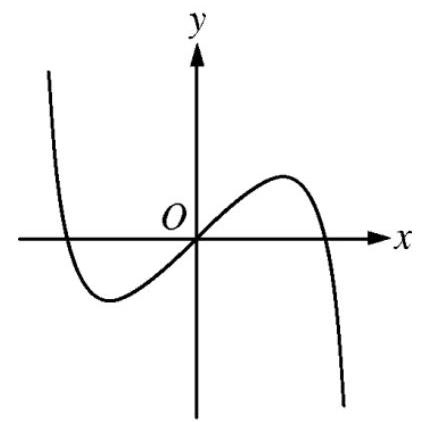
\includegraphics[width=1.41in]{media/9fa7ebca-42e0-529d-a9b6-bb493a83de14.jpg}\\
Which of the following could be the graph of \(f^{\prime}\), the
derivative of \(f\) ?
\vspace{1em}
		\begin{enumerate}
		\itemsep1em
			\item 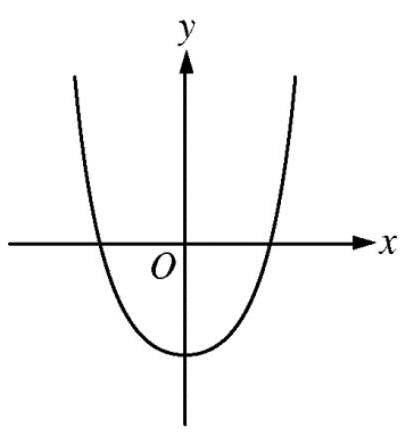
\includegraphics[width=1.38in]{media/67cece36-2bb7-5801-b710-e80e849bce43.jpg}
			\item 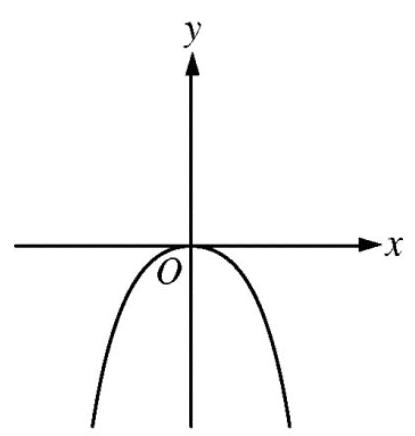
\includegraphics[width=1.3833333333333333in]{media/34b040f4-6501-5ae0-8cd3-c8435e7f9b34.jpg}
			\item 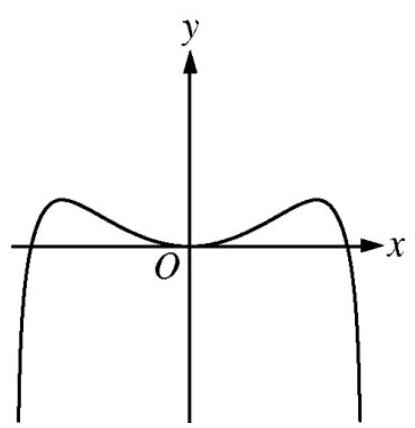
\includegraphics[width=1.3833333333333333in]{media/cc751a13-6b93-550d-a8de-7810aeda45df.jpg}
			\item 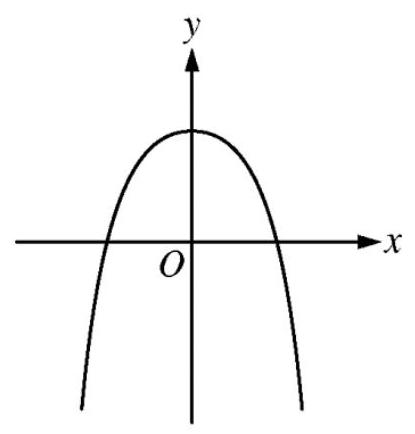
\includegraphics[width=1.3833333333333333in]{media/65b57584-1236-5154-956d-0f02bf998e7c.jpg}
			\item 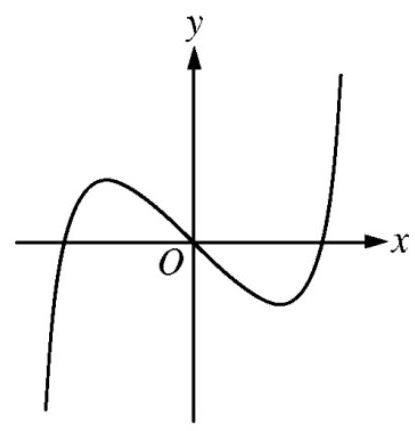
\includegraphics[width=1.3833333333333333in]{media/38af2d13-3933-571d-8f0d-39e0ec0fccc9.jpg}
		\end{enumerate}
	\end{minipage}
	\item
	\begin{minipage}[t]{\linewidth}
		Let \(h\) be the function defined by
\(h(x)=\int_{\pi / 4}^{x} \sin ^{2} t d t\). Which of the following is
an equation for the line tangent to the graph of \(h\) at the point
where \(x=\frac{\pi}{4}\) ?
\vspace{1em}
		\begin{enumerate}
		\itemsep1em
			\item \(y=\frac{1}{2}\)
			\item \(y=\sqrt{2} x\)
			\item \(y=x-\frac{\pi}{4}\)
			\item \(y=\frac{1}{2}\left(x-\frac{\pi}{4}\right)\)
			\item \(y=\frac{\sqrt{2}}{2}\left(x-\frac{\pi}{4}\right)\)
		\end{enumerate}
	\end{minipage}
	\item
	\begin{minipage}[t]{\linewidth}
		The number of people who have entered a museum on a certain day is
modeled by a function \(f(t)\), where \(t\) is measured in hours since
the museum opened that day. The number of people who have left the
museum since it opened that same day is modeled by a function \(g(t)\).
If \(f^{\prime}(t)=380\left(1.02^{t}\right)\) and
\(g^{\prime}(t)=240+240 \sin \left(\frac{\pi(t-4)}{12}\right)\), at what
time \(t\), for \(1 \leq t \leq 11\), is the number of people in the
museum at a maximum?
\vspace{1em}
		\begin{enumerate}
		\itemsep1em
			\item 1
			\item 7.888
			\item 9.446
			\item 10.974
			\item 11
		\end{enumerate}
	\end{minipage}
	\item
	\begin{minipage}[t]{\linewidth}
		A particle moves along a straight line with velocity given by
\(v(t)=5+e^{t / 3}\) for time \(t \geq 0\). What is the acceleration of
the particle at time \(t=4\) ?
\vspace{1em}
		\begin{enumerate}
		\itemsep1em
			\item 0.422
			\item 0.698
			\item 1.265
			\item 8.794
			\item 28.381
		\end{enumerate}
	\end{minipage}
	\item
	\begin{minipage}[t]{\linewidth}
		The function \(f\) is defined on the open interval \(0.4<x<2.4\) and has
first derivative \(f^{\prime}\) given by
\(f^{\prime}(x)=\sin \left(x^{2}\right)\). Which of the following
statements are true?

\begin{enumerate}[label=\Roman*.,leftmargin=1.0in]
  \item $f$ has a relative maximum on the interval $0.4<x<2.4$.
  \item $f$ has a relative minimum on the interval $0.4<x<2.4$.
  \item The graph of $f$ has two points of inflection on the interval $0.4<x<2.4$.
\end{enumerate}
\vspace{1em}
		\begin{enumerate}
		\itemsep1em
			\item I only
			\item II only
			\item III only
			\item I and III only
			\item II and III only
		\end{enumerate}
	\end{minipage}
	\item
	\begin{minipage}[t]{\linewidth}
		The first derivative of the function \(g\) is given by
\(g^{\prime}(x)=\cos \left(\pi x^{2}\right)\) for \(-0.5<x<1.5\). On
which of the following intervals is \(g\) decreasing?
\vspace{1em}
		\begin{enumerate}
		\itemsep1em
			\item \(-0.5<x<0\)
			\item \(0<x<1\)
			\item \(0.707<x<1.225\)
			\item \(1.225<x<1.414\)
			\item \(1.414<x<1.5\)
		\end{enumerate}
	\end{minipage}
	\item
	\begin{minipage}[t]{\linewidth}
		The height above the ground of a passenger on a Ferris wheel \(t\)
minutes after the ride begins is modeled by the differentiable function
\(H\), where \(H(t)\) is measured in meters. Which of the following is
an interpretation of the statement \(H^{\prime}(7.5)=15.708\) ?
\vspace{1em}
		\begin{enumerate}
		\itemsep1em
			\item The Ferris wheel is turning at a rate of 15.708 meters per minute when
the passenger is 7.5 meters above the ground.
			\item The Ferris wheel is turning at a rate of 15.708 meters per minute 7.5
minutes after the ride begins.
			\item The passenger's height above the ground is increasing by 15.708 meters
per minute when the passenger is 7.5 meters above the ground.
			\item The passenger's height above the ground is increasing by 15.708 meters
per minute 7.5 minutes after the ride begins.
			\item The passenger is 15.708 meters above the ground 7.5 minutes after the
ride begins.
		\end{enumerate}
	\end{minipage}
	\item
	\begin{minipage}[t]{\linewidth}
		Let \(f\) be a twice-differentiable function on the open interval
\((a, b)\). If \(f^{\prime}(x)>0\) on \((a, b)\) and
\(f^{\prime \prime}(x)<0\) on \((a, b)\), which of the following could
be the graph of \(f\) ?
\vspace{1em}
		\begin{enumerate}
		\itemsep1em
			\item 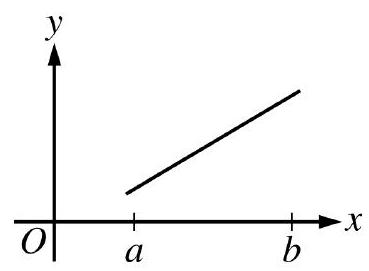
\includegraphics[width=1.23in]{media/e3a9f9b6-3a96-5d2d-add0-e6bd0546df0e.jpg}
			\item 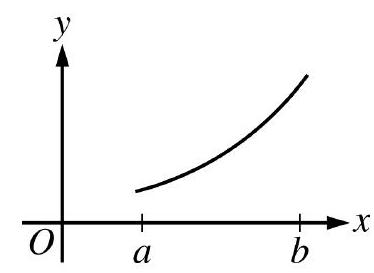
\includegraphics[width=1.2466666666666666in]{media/c548d8a9-e1c8-5b9b-ba75-6a9026b15b19.jpg}
			\item 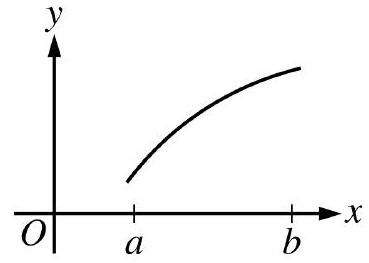
\includegraphics[width=1.23in]{media/254534e1-d2aa-57d9-be10-09a482f8eff8.jpg}
			\item 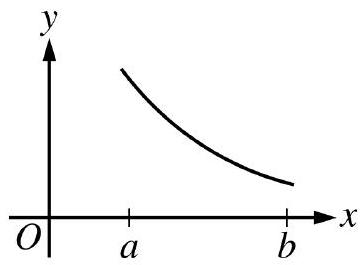
\includegraphics[width=1.2in]{media/c968da11-e2ba-553e-ad49-0df2477c4c35.jpg}
			\item 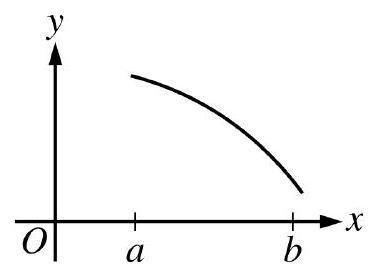
\includegraphics[width=1.2366666666666666in]{media/4d919db7-10f3-5dee-81b1-769c018bfad8.jpg}
		\end{enumerate}
	\end{minipage}
	\item
	\begin{minipage}[t]{\linewidth}
		In the \(x y\)-plane, the graph of the twice-differentiable function
\(y=f(x)\) is concave up on the open interval \((0,2)\) and is tangent
to the line \(y=3 x-2\) at \(x=1\). Which of the following statements
must be true about the derivative of \(f\) ?
\vspace{1em}
		\begin{enumerate}
		\itemsep1em
			\item \(f^{\prime}(x) \leq 3\) on the interval \((0.9,1)\).
			\item \(f^{\prime}(x) \geq 3\) on the interval \((0.9,1)\).
			\item \(f^{\prime}(x)<0\) on the interval \((0.9,1.1)\).
			\item \(f^{\prime}(x)>0\) on the interval \((0.9,1.1)\).
			\item \(f^{\prime}(x)\) is constant on the interval \((0.9,1.1)\).
		\end{enumerate}
	\end{minipage}
	\item
	\begin{minipage}[t]{\linewidth}
		Let \(f\) be the function given by \(f(x)=3-2 x\). If \(g\) is a
function with derivative given by
\(g^{\prime}(x)=f(x) f^{\prime}(x)(x-3)\), on what intervals is \(g\)
increasing?
\vspace{1em}
		\begin{enumerate}
		\itemsep1em
			\item \(\left(-\infty, \frac{3}{2}\right]\) and \([3, \infty)\)
			\item \(\left(-\infty, \frac{3}{2}\right]\) only
			\item \(\left[\frac{3}{2}, 3\right]\) only
			\item \(\left[\frac{3}{2}, \infty\right)\)
			\item \([3, \infty)\) only
		\end{enumerate}
	\end{minipage}
	\item
	\begin{minipage}[t]{\linewidth}
		A curve \(C\) is defined by the parametric equations \(x(t)=3+t^{2}\)
and \(y(t)=t^{3}+5 t\). Which of the following is an equation of the
line tangent to the graph of \(C\) at the point where \(t=1\) ?
\vspace{1em}
		\begin{enumerate}
		\itemsep1em
			\item \(y=\frac{1}{4} x+5\)
			\item \(y=4 x-10\)
			\item \(y=4 x+6\)
			\item \(y=8 x-26\)
			\item \(y=8 x+6\)
		\end{enumerate}
	\end{minipage}
	\item
	\begin{minipage}[t]{\linewidth}
		Let \(f\) be the function given by \(f(x)=x^{3}-2 x^{2}+5 x-16\). For
what value of \(x\) in the closed interval \([0,5]\) does the
instantaneous rate of change of \(f\) equal the average rate of change
of \(f\) over that interval?
\vspace{1em}
		\begin{enumerate}
		\itemsep1em
			\item 0
			\item \(\frac{5}{3}\)
			\item \(\frac{5}{2}\)
			\item 3
			\item 5
		\end{enumerate}
	\end{minipage}
	\item
	\begin{minipage}[t]{\linewidth}
		The position of a particle moving along the \(x\)-axis is given by a
twice-differentiable function \(x(t)\). If \(x(2)<0\),
\(x^{\prime}(2)<0\), and \(x^{\prime \prime}(2)<0\), which of the
following statements must be true about the particle at time \(t=2\) ?
\vspace{1em}
		\begin{enumerate}
		\itemsep1em
			\item The particle is moving toward the origin at a decreasing speed.
			\item The particle is moving toward the origin at an increasing speed.
			\item The particle is moving away from the origin at a decreasing speed.
			\item The particle is moving away from the origin at an increasing speed.
			\item The particle is moving away from the origin at a constant speed.
		\end{enumerate}
	\end{minipage}
	\item
	\begin{minipage}[t]{\linewidth}
		If \(0 \leq b \leq 2\), for what value of \(b\) is
\(\int_{0}^{b} \cos \left(e^{x}\right) d x\) a minimum?
\vspace{1em}
		\begin{enumerate}
		\itemsep1em
			\item 0
			\item 0.452
			\item 1.145
			\item 1.550
			\item 2
		\end{enumerate}
	\end{minipage}
	\item
	\begin{minipage}[t]{\linewidth}
		A cup has the shape of a right circular cone. The height of the cup is
\(12 \mathrm{~cm}\), and the radius of the opening is
\(3 \mathrm{~cm}\). Water is poured into the cup at a constant rate of
\(2 \mathrm{~cm}^{3} / \mathrm{sec}\). What is the rate at which the
water level is rising when the depth of the water in the cup is
\(5 \mathrm{~cm}\) ? (The volume of a cone of height \(h\) and radius
\(r\) is given by \(V=\frac{1}{3} \pi r^{2} h\).)
\vspace{1em}
		\begin{enumerate}
		\itemsep1em
			\item \(\frac{32}{25 \pi} \mathrm{cm} / \mathrm{sec}\)
			\item \(\frac{96}{125 \pi} \mathrm{cm} / \mathrm{sec}\)
			\item \(\frac{2}{3 \pi} \mathrm{cm} / \mathrm{sec}\)
			\item \(\frac{2}{9 \pi} \mathrm{cm} / \mathrm{sec}\)
			\item \(\frac{1}{200 \pi} \mathrm{cm} / \mathrm{sec}\)
		\end{enumerate}
	\end{minipage}
	\item
	\begin{minipage}[t]{\linewidth}
		A particle moves along the \(x\)-axis so that at time \(t \geq 0\) the
position of the particle is given by
\(x(t)=0.5 t^{4}-1.5 t^{3}-2 t^{2}+6 t-1\). What is the velocity of the
particle at the first instance the particle is at the origin?
\vspace{1em}
		\begin{enumerate}
		\itemsep1em
			\item -4.071
			\item -2.048
			\item 0
			\item 5.153
			\item 6
		\end{enumerate}
	\end{minipage}
	\item
	\begin{minipage}[t]{\linewidth}
		The graph of \(f^{\prime}\), the derivative of a function \(f\), is
shown below.\\
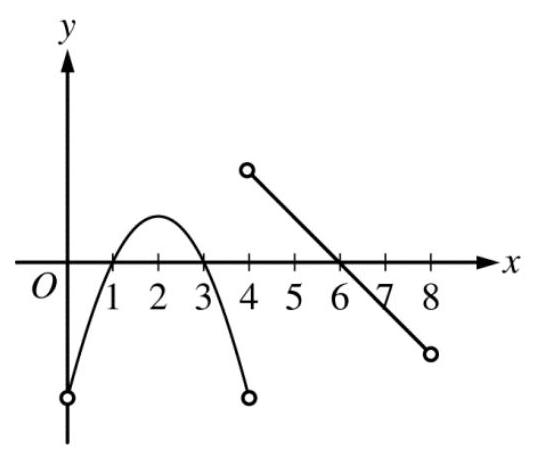
\includegraphics[width=1.78in]{media/8e560a60-029c-51b9-b81d-21c20bfc3c39.jpg}\\
Which of the following could be the graph of \(f\) ?

\begin{enumerate}[label=\Roman*.,leftmargin=1in]
    \item
    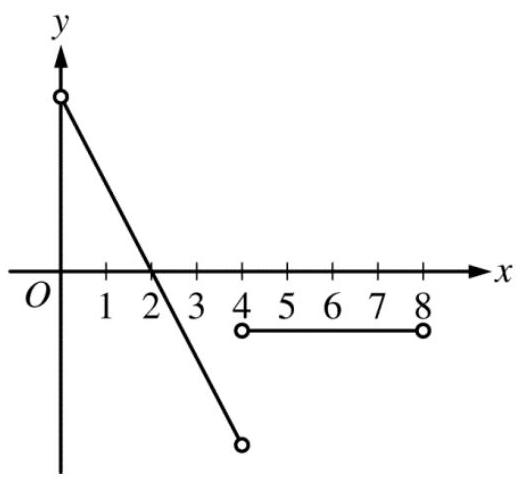
\includegraphics[width=1.7533333333333334in]{media/6612ab38-1aee-5b17-80ec-3d6b762222d9.jpg}
    \item
        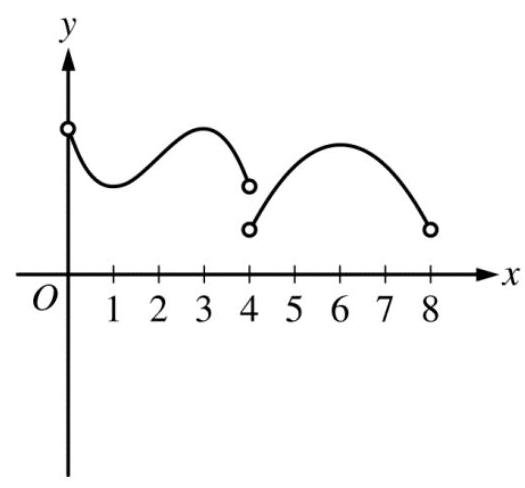
\includegraphics[width=1.75in]{media/b34aa28d-3cb2-53cf-8668-c2f9becbab45.jpg}
    \item
    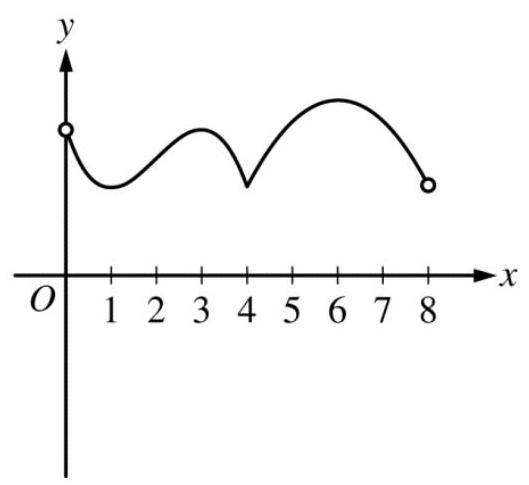
\includegraphics[width=1.7633333333333334in]{media/b6adf7c3-0019-5735-ae14-e1c3eb2a7a00.jpg}
\end{enumerate}
\vspace{1em}
		\begin{enumerate}
		\itemsep1em
			\item I only
			\item II only
			\item III only
			\item I and II only
			\item II and III only
		\end{enumerate}
	\end{minipage}
	\item
	\begin{minipage}[t]{\linewidth}
		The figure below\\
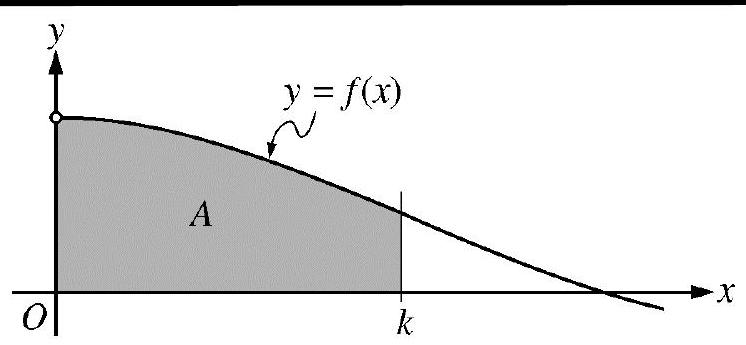
\includegraphics[width=2.486666666666667in]{media/2a75581e-08aa-568f-a673-3d320a67c403.jpg}\\
shows the region \(A\), which is bounded by the \(x\) - and \(y\)-axes,
the graph of \(f(x)=\frac{\sin x}{x}\) for \(x>0\), and the vertical
line \(x=k\). If \(k\) increases at a rate of \(\frac{\pi}{4}\) units
per second, how fast is the area of region \(A\) increasing when
\(k=\frac{\pi}{6}\) ?
\vspace{1em}
		\begin{enumerate}
		\itemsep1em
			\item 0
			\item \(\frac{3}{4}\)
			\item \(\frac{3}{\pi}\)
			\item \(\frac{\sqrt{3}}{2}\)
			\item \(2 \sqrt{3}\)
		\end{enumerate}
	\end{minipage}
	\item
	\begin{minipage}[t]{\linewidth}
		The number of gallons of water in a storage tank at time \(t\), in
minutes, is modeled by \(w(t)=25-t^{2}\) for \(0 \leq t \leq 5\). At
what rate, in gallons per minute, is the amount of water in the tank
changing at time \(t=3\) minutes?
\vspace{1em}
		\begin{enumerate}
		\itemsep1em
			\item 66
			\item 16
			\item -3
			\item -6
		\end{enumerate}
	\end{minipage}
	\item
	\begin{minipage}[t]{\linewidth}
		Let \(f\) be the function defined by \(f(x)=-3+6 x^{2}-2 x^{3}\). What
is the largest open interval on which the graph of \(f\) is both concave
up and increasing?
\vspace{1em}
		\begin{enumerate}
		\itemsep1em
			\item \((0,1)\)
			\item \((1,2)\)
			\item \((0,2)\)
			\item \((2, \infty)\)
		\end{enumerate}
	\end{minipage}
	\item
	\begin{minipage}[t]{\linewidth}
		A particle moves along the \(x\)-axis so that at time \(t>0\) its
position is given by \(x(t)=12 e^{-t} \sin t\). What is the first time
\(t\) at which the velocity of the particle is zero?
\vspace{1em}
		\begin{enumerate}
		\itemsep1em
			\item \(\frac{\pi}{4}\)
			\item \(\frac{\pi}{2}\)
			\item \(\frac{3 \pi}{4}\)
			\item \(\pi\)
		\end{enumerate}
	\end{minipage}
	\item
	\begin{minipage}[t]{\linewidth}
		The graph of \(f^{\prime}\), the derivative of the function \(f\), is
shown in the figure below.\\
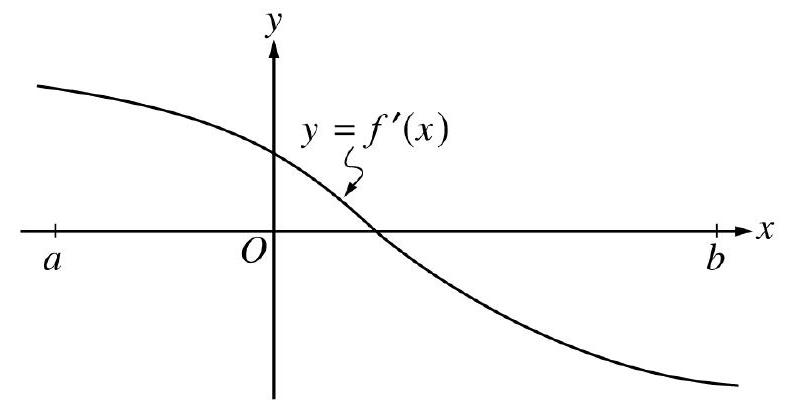
\includegraphics[width=2.62in]{media/3d1baae0-8207-59f4-922b-d9e10c1f8433.jpg}\\
Which of the following statements must be true?

\begin{enumerate}[label=\Roman*.,leftmargin=1in,topsep=1em]
    \item $f$ is continuous on the open interval $(a, b)$.
    \item $f$ is decreasing on the open interval $(a, b)$.
    \item The graph of $f$ is concave down on the open interval $(a, b)$.
\end{enumerate}
\vspace{1em}
		\begin{enumerate}
		\itemsep1em
			\item I only
			\item I and II only
			\item I and III only
			\item II and III only
		\end{enumerate}
	\end{minipage}
	\item
	\begin{minipage}[t]{\linewidth}
		An isosceles right triangle with legs of length \(s\) has area
\(A=\frac{1}{2} s^{2}\). At the instant when \(s=\sqrt{32}\)
centimeters, the area of the triangle is increasing at a rate of 12
square centimeters per second. At what rate is the length of the
hypotenuse of the triangle increasing, in centimeters per second, at
that instant?
\vspace{1em}
		\begin{enumerate}
		\itemsep1em
			\item \(\frac{3}{4}\)
			\item 3
			\item \(\sqrt{32}\)
			\item 48
		\end{enumerate}
	\end{minipage}
	\item
	\begin{minipage}[t]{\linewidth}
		The graph of a differentiable function \(f\) is shown in the figure
below\\
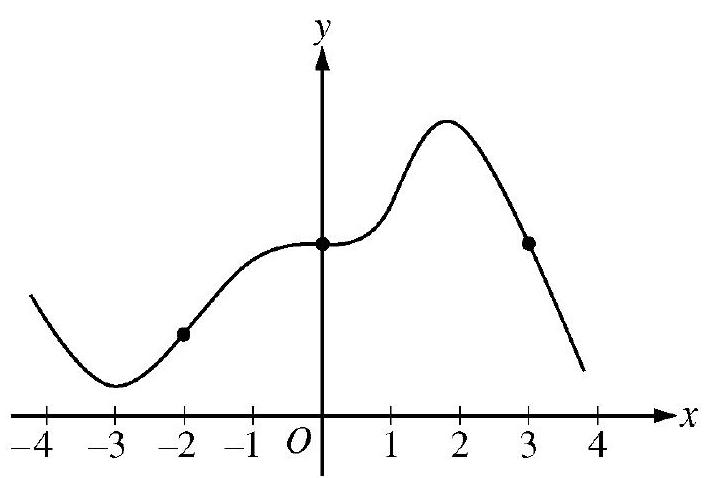
\includegraphics[width=2.3666666666666667in]{media/6c13bfc0-e550-5dba-b177-16d1151ff55a.jpg}\\
Which of the following is true?
\vspace{1em}
		\begin{enumerate}
		\itemsep1em
			\item \(f^{\prime}(-2)<f^{\prime}(0)<f^{\prime}(3)\)
			\item \(f^{\prime}(-2)<f^{\prime}(3)<f^{\prime}(0)\)
			\item \(f^{\prime}(3)<f^{\prime}(-2)<f^{\prime}(0)\)
			\item \(f^{\prime}(3)<f^{\prime}(0)<f^{\prime}(-2)\)
		\end{enumerate}
	\end{minipage}
	\item
	\begin{minipage}[t]{\linewidth}
		A file is downloaded to a computer at a rate modeled by the
differentiable function \(f(t)\), where \(t\) is the time in seconds
since the start of the download and \(f(t)\) is measured in megabits per
second. Which of the following is the best interpretation of
\(f^{\prime}(5)=2.8\) ?
\vspace{1em}
		\begin{enumerate}
		\itemsep1em
			\item At time \(t=5\) seconds, the rate at which the file is downloaded to the
computer is 2.8 megabits per second.
			\item At time \(t=5\) seconds, the rate at which the file is downloaded to the
computer is increasing at a rate of 2.8 megabits per second per second.
			\item Over the time interval \(0 \leq t \leq 5\) seconds, 2.8 megabits of the
file are downloaded to the computer.
			\item Over the time interval \(0 \leq t \leq 5\) seconds, the average rate at
which the file is downloaded to the computer is 2.8 megabits per second.
		\end{enumerate}
	\end{minipage}
\end{enumerate}




\end{document}
